\glsresetall
 \graphicspath{{figures/analysing/}}
\chapter{Introduction}

The directivity of a sound sources is an issue that has an impact on many situations of our daily life, e.g. at live music venues. Voluntary listeners, namely the audience, enjoy comparatively high sound pressure levels when gathering around the stage. Non-voluntary listeners, generally neighbours, tend to perceive the sound emitted by the stage as a disturbing noise. This problem might be minimized with directivity control of the sound sources. The high sound energy will then be emits towards the audience, and less towards the neighbours. 


There are several effects that make this difficult, because commonly used loudspeaker contraptions for low frequency playback tend to act like omnidirectional sound sources. First, the dampening of sound in the air has significantly less influence on sound towards the lower frequency of the human hearing range than it has towards the higher frequency. Secondly, because of the way most houses are built, low frequency sound penetrates through walls and windows much more than high frequency sound. All of these effects lead to neighbours being disturbed by \textit{the low frequency} from nearby live music venues.\\
The difference in the perception of the sound is visualised in \autoref{fig:Problem}.


\begin{figure}[htbp]
	\centering
	\includegraphics[width=1\textwidth]{change_later.png}
	\caption{Normalized \gls{spl} in colour, red is high \gls{spl} where blue is low \gls{spl}}
		\label{fig:Problem}
\end{figure}

%\autoref{fig:Problem} shows the total sound pressure level \gls{spl} in \gls{db} from \SI{20}{\hertz} to \SI{20}{\kilo\hertz} for the voluntary listeners and the non-voluntary listeners during a concert.
\autoref{fig:Problem} shows a qualitative drawing of a near-ideal sound pressure distribution in the vicinity of a stage during a concert. The high-\gls{spl}areas are highlighted by red color, and is the area where the voluntary listeners condense. This area is define as the \textbf{participants' area} The non-voluntary listeners are located in the area around the participants' area, that we define as \textbf{the neighbourhood}. 

While a \gls{spl} distribution as depicted in \autoref{fig:Problem} is easier to achieve the higher the frequency gets, towards low frequencies the \gls{spl}distribution might look more like depicted in autoref(fig:problem2).



The directivity control of mid- and high frequency has a known solution which has been applied for many years. In general, horns are used, which are designed for a particular radiation pattern. Due to the long wave length in the low/mid- and low frequency range, the horns that are required to direct those wavelengths are not feasible for practical applications due to their size and weight. Therefore other, more space saving solutions have been developed and implemented in the last decade. It is possible to achieve a cardiod emission pattern by arranging subwoofers in a particular manner. Two or three subwoofers are pointed towards the participants' area and one subwoofer is pointed the opposite way. The signal for the subwoofer pointing away from the audience is processed to manipulate the phase.


This project aims towards applying a principle that has been put into commercial use in the D\&B audiotechnik SL-series, where the low/mid frequency directivity is controlled by signal processing four speaker unit. Two units are arranged in the front of the line array module and the other two arranged on each of the sides of the line array module.



\section{preliminary problem statement}
The following questions are made with the intention of gathering the necessary knowledge, to be able to answer a later stated problem statement. The preliminary questions, which will be answered in the analysis, are:

\begin{itemize}
\item In which frequency area do the line source speaker behave omnidirectional?
\item Which known technique is used to do the speaker cardioid?
\item Can a simulation be made which support D\&B audiotechnik claim?
\end{itemize}




%%%
\part{Problem Analysis}\label{pt:analysis} \glsresetall
 \graphicspath{{figures/analysing/}}
	\chapter{Directional characteristics of a loudspeaker}\label{ch:directional}
		\section{Origin}
Because this project is about shaping the directional characteristics of loudspeakers arrangements towards a particular direction, it is important to thorougly investigate the directional characteristic of a single loudspeaker cabinet. This serves as a baseline for comparison and also is essential, because the investigated cabinet will be used to form the speaker array later on.\\
In general, loudspeakers tend to display different directional behaviour depending on the frequency emitted. At low frequencies they can be viewed as omnidirectional sound sources. At higher frequencies the main direction of sound emission is in line with the motion direction of the voice coil. \citep{crocker98}
Depending on the ratio of the emitted wavelength to the diameter of the speaker, a radiation pattern with side lobes can occur. An analytic approximation to the behaviour can be made  when looking at a vibrating piston in an infinite baffel. However, this only takes into account the front side of the speaker. It is difficult to incorporate the effects of an enclosure into this model.\\
There are possibilities to numerically model the sound field around a speaker in a cabinet. However in the context of this project, conducting a measurement seems to be the most favourable approach towards quantifying the sound emitted by loudspeaker in the cabinet at numerous frequencies.
The knowledge gained through the measurements can then be used in order to designate a feasible frequency range for the beamforming.
	\chapter{Analytical descriptions}\label{ch:analytical}
		\section{Single source}\label{ch:single_speaker_source}
To gain understanding about the interaction of several sources emitting sound simultaneously it is essential to first investigate the behaviour of a single sound source. In the context of this project loudspeakers are investigated. The goal of this section is to find a way to represent the sound emission of loudspeakers within the frequencies boundaries of this project (\SIrange{60}{300}{\hertz}).
The representation must be suffiencently accurate yet relatively simple to calculate in order to be useful in the optimization process that is a later part of this project (see \autoref{ch:optimization}).

%This section aims to introduce and analyse the fundamental for a single source, by analyse the behaviour of a baffled circular plane piston source. The pressure around the piston source will be analysed analytically, to determine the radiation of a single speaker from \SI{60}{\hertz} and upwards and compare it with the measurement from \autoref{ch:polar_response}. The \SI{60}{\hertz} lower limit enable the simulation to be validated by measurement in the AAU anechoic chamber and is a used lower limit for the low/mid driver in some line source array \citep{V-DOSC}.  The analyse shall end out with a approximated simulation model of the \gls{dut}.
\subsection{Pressure emission from an omidirectional source}\label{ssec:omni}
As explained in \autoref{ch:polar_response} loudspeakers are commonly treated as omnidirectional sources at low frequencies. Taking advantage of this approximation, the sound pressure emission in free field conditions can be described conveniently. \citep[p. 171]{Kinsler2000} state the following equation \autoref{eq:omni_source} for a pulsating sphere. It has to be noted, that the position of the sphere in the given case is the acoustic center of the loudspeaker (see \autoref{sec:ac_center}).
\begin{equation}\label{eq:omni_source}
p(r,t)\,=\,\rho_0 c V_0 \left(\frac{a}{r}\right)\cos \theta_a \textbf{\textit{e}}^{j\left(\omega t - k(r-a)+\theta_a\right)}
\end{equation}
\startexplain
\explain{$p$ is the sound pressure.}{\si{\pascal}}
\explain{$r$ is the distance, for which the pressure is being calculated, \(r>a\).}{\si{\meter}}
\explain{$t$ is the time, for which the pressure is being calculated.}{\si{\meter}}
\explain{$\rho_0$ is the specific density of air.}{\si{\kilo\gram\per\cubic\meter}}
\explain{$c$ is the speed of sound.}{\si{\meter\per\second}}
\explain{$V_0$ ist the peak velocity at the surface of the spherical source.}{\si{\meter\per\second}}
\explain{$a$ is the radius of the spherical source.}{\si{\meter}}
\explain{$\theta_a$ is equal to $\tan(ka)$.}{\si{1}}
\explain{$\omega$ is the angular frequency.}{\si{\second^{-1}}}
\explain{$k$ is the wavenumber.}{\si{\meter^{-1}}}
\stopexplain

\subsection{Pressure emission from a baffled piston}\label{ssec:piston}
Another  approach to analytically approximate the behaviour of a cone loudspeaker is given by \citep[p. 179 ff.]{Kinsler2000}, where the behaviour of the sound radiated from a plane circular piston surrounded by an infinte rigid baffle is described. The piston model is derived from the model of a continous line source as described in \citep[p. 176 f.]{Kinsler2000}.


%To characterize the directional properties of an analytical model of the \gls{dut}, the source will be modulated in two dimension as one baffled circular plane piston source. The analysis of a piston source in two dimension built on a thin piston source in three dimension where the x axis is fixed in the plot. This is possible because of vertical beam patten symmetry of \autoref{fig:continues_line_source} \citep{Kinsler2000}. The piston lays flat down so i look like a line source and have radius $a$. The baffled circular plane piston source can be considered as many continuous line sources, which detonate dx and is pointing towards the reader on \autoref{fig:continues_line_source}. The calculated pressure point will be in far field where $r>>a$ holds and the surface integral can be rewritten to a Bessel function \citep{Kinsler2000}. The pressure formula is therefore:

\begin{equation}\label{eq:piston_source}
p(r,\theta ,t)=\frac{j}{2} \rho_{0}c  V_{0}\frac{a}{r}ka \left ( \frac{2J_1(ka\, sin(\theta ))}{ka\, sin(\theta )} \right )e^{j(\omega t-kr)}
\end{equation}
\startexplain
	\explain{$r$ is the distance, for which the pressure is being calculated, \(r>a\).}{\si{\meter}}
	\explain{$\theta$ is the angle at which the pressure is calculated, relative to the direction, in which the piston is moving.}{\si{1}}
	\explain{$t$ is the time, for which the pressure is being calculated.}{\si{\meter}}
	\explain{$j$ is the imaginary unit}{\si{1}}
	\explain{$\rho_0$ is the specific density of air.}{\si{\kilo\gram\per\cubic\meter}}
	\explain{$c$ is the speed of sound.}{\si{\meter\per\second}}
	\explain{$V_0$ ist the peak velocity of the piston.}{\si{\meter\per\second}}
	\explain{$a$ is the radius of the piston.}{\si{\meter}}
	\explain{$k$ is the wavenumber.}{\si{\meter^{-1}}}
	\explain{$J_1$ is the Bessel function of the first kind of order 1.}{\si{1}}
	\explain{$\omega$ is the angular frequency.}{\si{\second^{-1}}}
\stopexplain

A major disadvantage to utlizing the piston model in the context of the project is, that no information about the cabinet of the \gls{dut} is incorporated. The concept of an infinite rigid baffle leads to results that are axis symmetric along the \SIrange{-90}{90}{\degree}-line in a polar plot. This is illustrated in \autoref{fig:piston_analytical}.
\begin{figure}[H]
	\centering
	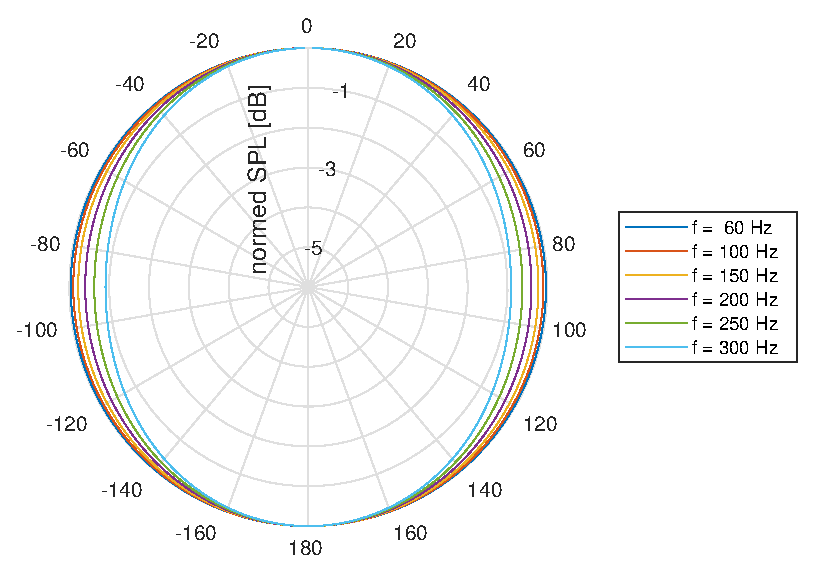
\includegraphics[width=0.7\textwidth]{piston.eps}
	\caption{normed SPL according to \autoref{eq:piston_source}, $a=165.3$\si{\milli\meter}$\,\approx 13$'', corresponding to the size of \citep{seas33}.}
		\label{fig:piston_analytical}
\end{figure}
\autoref{fig:piston_analytical} displays almost perfect omnidirectional behaviour for lower frequencies and lowering pressure towards $\pm$\SI{90}{\degree} for higher frequencies. The deviation from omnidirectionality has the same qualitative appearance as the measured pressure curves in \autoref{fig:03_02_pressure_main}, however they significantly differ in numbers.
\begin{figure}[htbp]
	\centering
	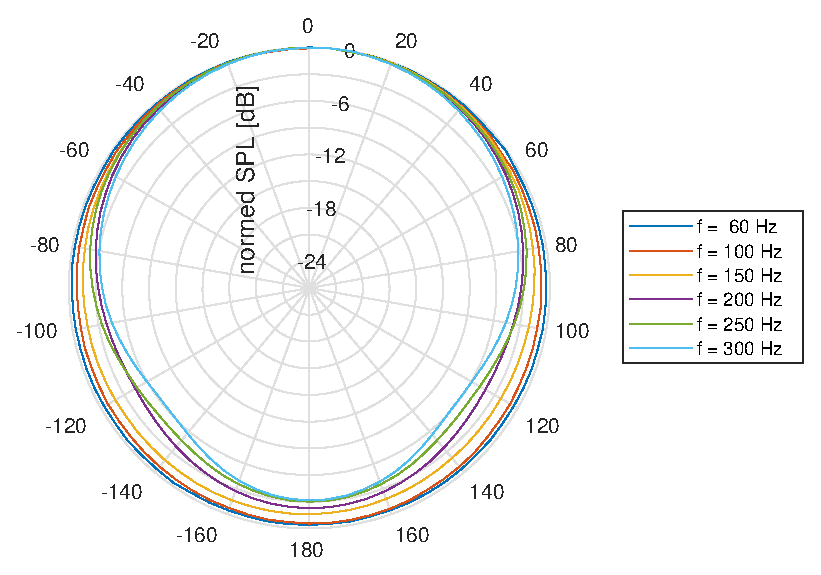
\includegraphics[width=0.7\textwidth]{03_02_meas1_pressure.eps}
	\caption{Normed \gls{spl}, measured at a distance \(d=\)\SI{2.74}{\meter}, see Appendix \ref{ax:directional_2}}
		\label{fig:03_02_pressure_main}
\end{figure}
\autoref{fig:03_02_pressure_main} also illustrates, that the solutions obtained with \autoref{eq:piston_source} do not realistically represent how the pressure is emitted on the back side of the speaker. Specifically, the indents in the in the curves for frequencies $\ge$\SI{200}{\hertz} at approx. $\pm$\SI{125}{\hertz} in \autoref{fig:03_02_pressure_main} deviate from the shape that is drawn by the piston model.
%The movement of the surface is described with

%\begin{equation}
%v = V_{0} \cdot exp(j \omega t)
%\end{equation}

%\startexplain
%    	\explain{$v$ is the complex speed of the line source }{\si{1}}
%        \explain{$V_{0}$ is the Amplitude}{\si{1}}
%        \explain{$j$ is the imaginary unit }{\si{1}}
%        \explain{$\omega$ is the angular velocity }{\si{1}}
%        \explain{$t$ is the time }{\si{1}}
%\stopexplain
    
%Each small sources is treated as an baffled simple source with a width of $dx$ and the source strange can be modulated as following      
%
%\begin{equation}
%dQ = V_{0} 2 a\, sin(\phi) \, dx
%\end{equation}
%
%    \startexplain
%    		\explain{$dQ$ is the simple source strange }{\si{1}}
%        \explain{$V_{0}$ is the Amplitude}{\si{1}}
%        \explain{$a$ is the radius for cylinder }{\si{1}}
%        \explain{$\phi$ is the angle between the radius $a$ and the x axis}{\si{1}}
%        \explain{$dx$ is the length for the simple source }{\si{1}}
%    \stopexplain    
% 
%The following \autoref{fig:continues_line_source} shows an example of the continues line source where one of the small source is showed with width $dx$ and length $2a \, sin(\phi)$. 
%
%\begin{figure}[H]
%	\centering
%\begin{picture}(0,0)%
%\includegraphics{line_source.pdf}%
%\end{picture}%
%\setlength{\unitlength}{746sp}%
%%
%\begingroup\makeatletter\ifx\SetFigFont\undefined%
%\gdef\SetFigFont#1#2#3#4#5{%
%  \reset@font\fontsize{#1}{#2pt}%
%  \fontfamily{#3}\fontseries{#4}\fontshape{#5}%
%  \selectfont}%
%\fi\endgroup%
%\begin{picture}(31223,16833)(-5411,-436)
%\put(12106,7139){r'}%
%\put(24121,15599){P(r,$\theta$,t)}%
%\put(946,2684){$\theta$}%
%\put(23851,659){x}%
%\put(-89,16094){z}%
%\put(11341,8354){r}%
%\put(3466,-571){$a$}%
%\put(1441,-376){$dx$}%
%\put(-134,-421){0}%
%\put(-4049,-571){$-a$}%
%\put(226,1649){$\Delta$r}%
%\end{picture}%
%	\caption{The model of a continues line source where y axis is pointing towards the reader. (ref the book)}
%		\label{fig:continues_line_source}
%\end{figure}




%\subsection{Comparison: calculations based on the baffled piston and measured polar respone}
%In this section, the \gls{dut} will be simulated as a baffled circular plane piston source as described in \autoref{ch:single_speaker_source} and compared to the actually measurement of the \gls{dut} \autoref{ax:directional_2}. An piston simulated model of \citep{seas33} in MATLAB shows in \autoref{fig:piston_model_of_seas33}
%
%\begin{figure}[H]
%	\centering
%	\includegraphics[width=0.8\textwidth]{piston_model.pdf}
%	\caption{The figure shows  The \gls{dut} which correspond to this figure is a \citep{seas33}}
%		\label{fig:piston_model_of_seas33}
%\end{figure}
%
%The actually measurement of the \citep{seas33}  \autoref{ax:directional_2}.
%
%\begin{figure}[H]
%	\centering
%	\includegraphics[width=0.8\textwidth]{meas1_seas.pdf}
%	\caption{The figure shows  The \gls{dut} which correspond to this figure is a \citep{seas33}}
%		\label{fig:speaker_model}
%\end{figure}

\subsection{Fitting the omnidirectional source model to the \gls{dut}}\label{sec:correction}
The analytical descriptions of both the pulsating sphere (see \autoref{ssec:omni}) and the piston (see \autoref{ssec:piston}) do not describe the measured behaviour of the \gls{dut} in an adequate manner. In order to be able to perfom an optimization of the signal processing parameters for the speaker array (see \autoref{ch:optimization}), a sufficient model has to be obtained. For the sake of this project, it has been chosen to rely on measured data.
As the pressure and phase characteristic of the \gls{dut} have been ascertained in measurements (see Appendices \ref{ax:directional_1},\ref{ax:directional_2}), the measurements results can be processed to obtain a correction table relating to the model of the omnidirectional source. This is achieved by calculating a difference of the measured data from the ideal values, that would suggest omnidirectionality at any given frequency. The resolution of the correction grid is determined by angular resolution and the frequency resolution of the polar response measurement, that it is based on.  \autoref{fig:correction_3d} shows a pressure correction grid, based on the polar response from Appendix \ref{ax:directional_2}.
\begin{figure}[H]
	\centering
	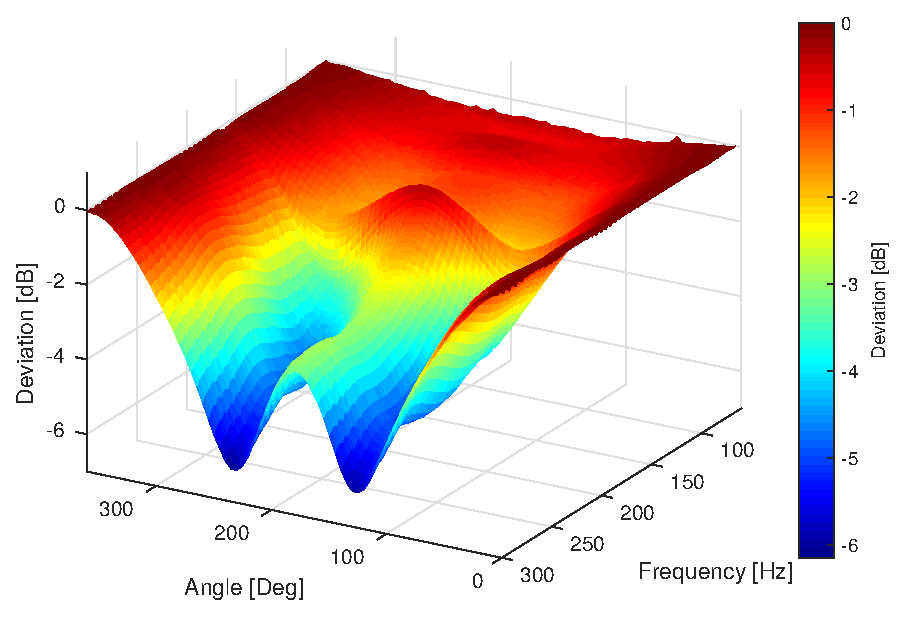
\includegraphics[width=0.7\textwidth]{correction_3d.eps}
	\caption{Contour plot of the pressure correction data, based on measurement data from Appendix \ref{ax:directional_2}}
		\label{fig:correction_3d}
\end{figure}
With the correction values applied, an augmented form of \autoref{eq:omni_source} can be established. Note, that while the deviation from omnidirectionality is visualized in \autoref{fig:correction_3d} in a \si{\decibel}-scale, for the usage in the \textsf{Dev}-function in \autoref{eq:aug_omni}, data has to be presented linearly.
\begin{equation}\label{eq:aug_omni}
p(r,t)\,=\,\rho_0 c V_0 \left(\frac{a}{r}\right)\cos \theta_a \textbf{\textit{e}}^{j\left(\omega t - k(r-a)+\theta_a\right)}\cdot\textsf{Dev}(f,\phi)
\end{equation}
\startexplain
\explain{$p$ is the sound pressure.}{\si{\pascal}}
\explain{$r$ is the distance, for which the pressure is being calculated, \(r>a\).}{\si{\meter}}
\explain{$t$ is the time, for which the pressure is being calculated.}{\si{\meter}}
\explain{$\rho_0$ is the specific density of air.}{\si{\kilo\gram\per\cubic\meter}}
\explain{$c$ is the speed of sound.}{\si{\meter\per\second}}
\explain{$V_0$ ist the peak velocity at the surface of the spherical source.}{\si{\meter\per\second}}
\explain{$a$ is the radius of the spherical source.}{\si{\meter}}
\explain{$\theta_a$ is equal to $\tan(ka)$.}{\si{1}}
\explain{$\omega$ is the angular frequency.}{\si{\second^{-1}}}
\explain{$k$ is the wavenumber.}{\si{\meter^{-1}}}
\explain{$\textsf{Dev}$ is the pressure deviation from the correction table.}{\si{1}}
\explain{$f$ is the frequency.}{\si{\hertz}}
\explain{$\phi$ is the angle, for which the pressure is being calculated relative to the main axis of the speaker.}{\si{1}}
\stopexplain
\section{Conclusion of single source}
Investigating analytical ways to express the behaviour of a speaker by incorporation no other information then its size leads to results that are not particulary accurate and are therefore of limited use. While it appears to be possible to get better estimates by incorporating more information into a numerical model (e.g. \citep{vanderkooy10}). The given objective of using the model for an optimization makes this approach unfeasible. Because measurements have been conducte investigating the directional characteristics of the loudspeaker that will later be used, a more empirical approach has been found. Exploiting information from the measurements, the relatively simple model of a pulsating sphere can be augmented, so that it fits the behaviour of the \gls{dut}.
		\section{The 300 \gls{hz}}
		\input{chapters/analysing/dimension_limit}
	\chapter{Numerical Simulation}\label{ch:numerical}   



%%
\part{Design and Optimization}\label{pt:design} 
\graphicspath{{figures/design/}}
	\chapter{Hardware Configuration}
		%\input{chapters/design/dspchoice}
	\chapter{Optimizing SP-Parameters}
	\chapter{Implementing SP-Parameters}


%%

\part{Test and Discussion}\label{pt:test}
\graphicspath{{figures/tests/}}
	\chapter{Performance Evaluation}
		%\input{chapters/tests/test_intro}
	\chapter{Comparison: Simulations and Measurement}
	\chapter{Comparison: Array vs Single Speaker}


 
%%
\part{Conclusion}\label{pt:conclusion}
%\chapter{Discussion}
\section{Comparison to a Commercial Product}
In order to get an idea of what directional characteristics have been achieved by others, the beamforming array is compared to a line array unit by the company D\&B, who specifically use their directivity control for marketing. The so called GLS8 unit is depicted in \autoref{fig:gls8_pic}. For the frequency range of this project, the key data is, that in the line array unit, two 14$^{\prime \prime}$ drivers in the front of the unit are placed, and another two 10$^{\prime \prime}$ drivers are mounted in the sides \citep{SL_GSL}[p. 6]. 
\begin{figure}[H]
\centering
\includegraphics[width=0.4\textwidth]{sl8.png}
\caption{Drawing of D\&B GLS8 line array unit, image source: \citep{SL_GSL}[p. 6]}
\label{fig:gls8_pic}
\end{figure}
The directional characteristics of the GSL8 units are depicted in \autoref{fig:gls_iso}. 
It has to be noted that this plot covers a significantly wider frequency range, than the one featured in this project. Between \SI{200}{\hertz} and \SI{300}{\hertz}, the line array unit clearly has a smaller \SI{-6}{\decibel} lobe width (approx. \SI{80}{\degree}) than the triangular array (approx. \SI{140}{\degree}), which is featured in \autoref{fig:array_iso}.
\autoref{fig:gls_iso} shows, that the lobe width for the line array module has a tendency to grow with decreasing frequency. At \SI{63}{\hertz} the \SI{-6}{\decibel} lobe width of the GSL8 unit is approx. \SI{144}{\degree}, which is in the same order of magnitude as the approx. \SI{150}{\degree} lobe width of the triangular array. When looking at these plots it has to be taken into account, that the two constructions were designed to fulfill different requirements and have very different cabinet configurations. It might be speculated, that perhaps the relatively large single cabinet of the line array unit aids directionality at higher frequencies, where at the lower end of the frequency band more of the directionality control has to be achieved by beamforming. This would explain, why at higher frequencies the lobe width of the GSL8 is clearly superior to the triangular array, while they both have similar characteristics around \SI{60}{\hertz}.
\begin{figure}[H]
\centering
	\begin{subfigure}[H]{0.7\textwidth}
		\centering
		\includegraphics[width=0.95\textwidth]{gls_isobar.png}
		\subcaption{Isobar plot for the GSL8 module, showing \SI{-6}{\decibel} and \SI{-12}{\decibel} isobars, image source: \citep{SL_GSL}[p. 9]}	
		\label{fig:gls_iso}
	\end{subfigure}\\
	\begin{subfigure}[H]{0.95\textwidth}
		\centering
		\includegraphics[width=0.95\textwidth]{dbcompare.eps}
		\subcaption{Contour plot of the relative level over frequency and angle for the triangular speaker array. Modified version of \autoref{fig:beamdwidth_array_on}, with resolution adjusted for comparison}
		\label{fig:array_iso}
	\end{subfigure}
\caption{Directional characteristics, GSL8 and triangular speaker array.}
\label{fig:isobars}
\end{figure}
\section{Applications}\label{sec:applications}
\subsection{Home application}
The beamforming array might be quite big for home application, but it may be possible to reduce the size of the beamforming array with smaller speaker units. At this point there are several possibility for home application. Imagen that the house is designed and built as an open living environment, where the kitchen and the living room is a combined open area. There might be a television with stereo speakers in the living room where the back for the television and the back of speaker points towards the kitchen. The low frequency might be an issue backwards because a low frequency driver radiate omnidirectional. At higher frequency the power is more radiated agents the person that watch television, because the high frequency driver is cardioid in it self, only the reflection reflect back to the kitchen. Because of this directionality, there might be higher pressure in the kitchen of the low frequency than the high frequency. Therefore the sound might be annoying in the kitchen because it is dominated by the low frequency. A simulation of a indoor situation with 2 speaker array is a living room is done in \autoref{fig:Indoor_simulation_60_100} and \autoref{fig:Indoor_simulation_200_300}
 




\subsection{Monitoring}
Using a normal loudspeaker as a stage monitor might lead to some complications, where the monitor and the microphone create a feedback loop or the performer is ignored by the neighbour performer monitor. The beamforming array cannot solve the feedback loop, but the beamforming array will lower the pressure in side of the monitor at low frequency and might have an useful effect. This application both have a posential at stage inside and outside. The problem of using this inside can be that the reflection is so strong that the effect do not work as intended. Another problem with monitor might be that the stage is small and there is barely space for the monitor. By adding additional input and filter for different direction of the beamforming array, it might be possible to take away three monitors and replace them by one beamforming array on such small stage. By narrow the front beam and allow higher beam at the back the sound might be possible to point on the performer as wanted. This kind of bemforming require further investigation and designing which not is done in this project. A simulation is made of a indoor application where two monitors of the beemforming array are placed on a stage, see \autoref{sec:dis:simulation}



\subsection{Main application}
The main application of the beamforming array was intended to outdoor venue, where the neighbour was the non voluntary listener. In this application where the speaker is under free field condition, it have been shown that the sound pressure can be attenuated at least \SI{-9}{\decibel} at the back and side of the array. Therefore the beamforming array will help damping the this kind of side effect of outdoor concert.


\subsection{Simulation}\label{sec:dis:simulation}
The aim of this section is to shortly investigate the wave behaver of the speaker array inside with wall reflection. This project have covered the design of the beamforming array and the behaver in free field condition. The indoor application have been keep out of interest, because of the starting point of application, which have been focused on outdoor event. The last point in the introduction was questioning the indoor application of the beamforming array. At this point there is many possibility since every room is different. The room could be a big concert hall or just a small room for living. It have been chosen to simulate a concert hall because of the monitoring application and the living room for home application. For the living room, it have been chosen to use a standard listening room of size (\SI{4.15}{\meter} x \SI{7.8}{\meter}) which correspond to the \gls{aau} standard listening room. All simulation will be done in 2 dimension because of the computation time and memory requirement. It will not give the exact simulation of the room, but since the reflection coefficient of the room wall not is measured there is already many unknown parameters in this simulation. The reflection in this simulation is done where the $Z_{-1}$ and $Z_{1}$ is unknown and set to zero, because in many case the characteristic wall impedance $Z_0$ is the predominant part \citep{fdtd_imp}. $Z_0$ can be approximated with using the absorbing coefficient \citep{fdtd_imp}. The following \autoref{eq:absorb} shows the approximated characteristic wall impedance $Z_0$ calculation

\begin{equation}\label{eq:absorb}
Z_0 = \rho c \frac{1+\sqrt{1-\alpha}}{1-\sqrt{1-\alpha}}
\end{equation}

        \startexplain
        \explain{$a$ is the absorbing coefficient}{\si{1}}
    \stopexplain
    
 The simulation give an impression of the wave behaviour in the room and not valid result. The result from a simulation of a size like the listening room is shown in \autoref{fig:Indoor_simulation_60_100} and \autoref{fig:Indoor_simulation_200_300}



\begin{figure}[H]
\begin{subfigure}[c]{0.5\textwidth}
\includegraphics[width=0.95\textwidth]{60_hz_inside_beam.eps}
\subcaption{Indoor simulation of  \SI{60}{\hertz} with beamforming}
\label{fig:Indoor_simulation_60_on}
\end{subfigure}
\begin{subfigure}[c]{0.5\textwidth}
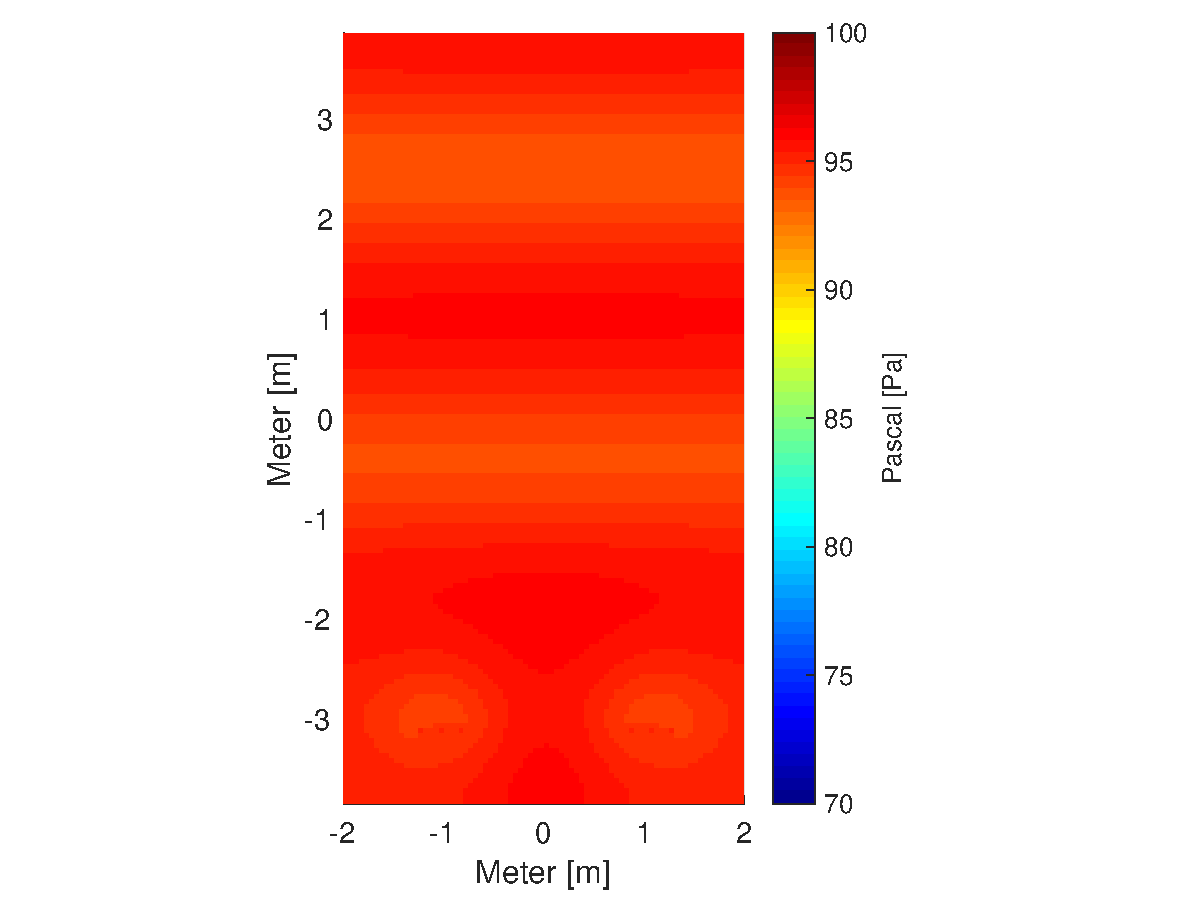
\includegraphics[width=0.95\textwidth]{60_hz_inside_without_beam.eps}
\subcaption{Indoor simulation of  \SI{60}{\hertz} without beamforming}
\label{fig:Indoor_simulation_60_off}
\end{subfigure}\\
\hspace{0.1\textheight}
\begin{subfigure}[c]{0.5\textwidth}
\includegraphics[width=0.95\textwidth]{100_hz_inside_beam.eps}
\subcaption{Indoor simulation of  \SI{100}{\hertz} with beamforming}
\label{fig:Indoor_simulation_100_on}
\end{subfigure}
\begin{subfigure}[c]{0.5\textwidth}
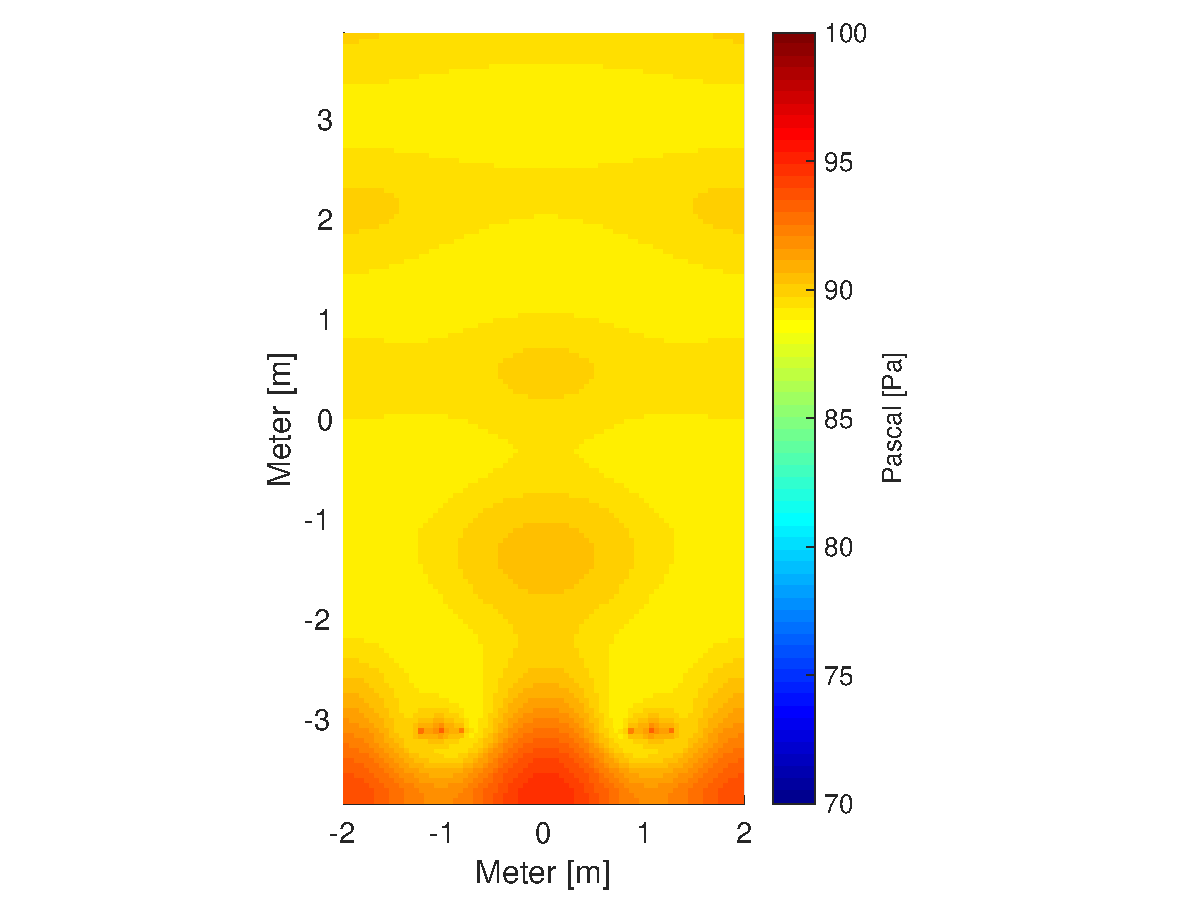
\includegraphics[width=0.95\textwidth]{100_hz_inside_without_beam.eps}
\subcaption{Indoor simulation of  \SI{100}{\hertz} with beamforming}
\label{fig:Indoor_simulation_100_off}
\end{subfigure}
\caption{The figure shows a 2 dimension \gls{fdtd} simulation in a room of size  (\SI{4.15}{\meter} x \SI{7.8}{\meter}) where the absorbing coefficient is set to 0.5}
		\label{fig:Indoor_simulation_60_100}
\end{figure}


\begin{figure}[H]
\begin{subfigure}[c]{0.5\textwidth}
\includegraphics[width=0.95\textwidth]{200_hz_inside_beam.eps}
\subcaption{Indoor simulation of  \SI{200}{\hertz} with beamforming}
\label{fig:Indoor_simulation_200_on}
\end{subfigure}
\begin{subfigure}[c]{0.5\textwidth}
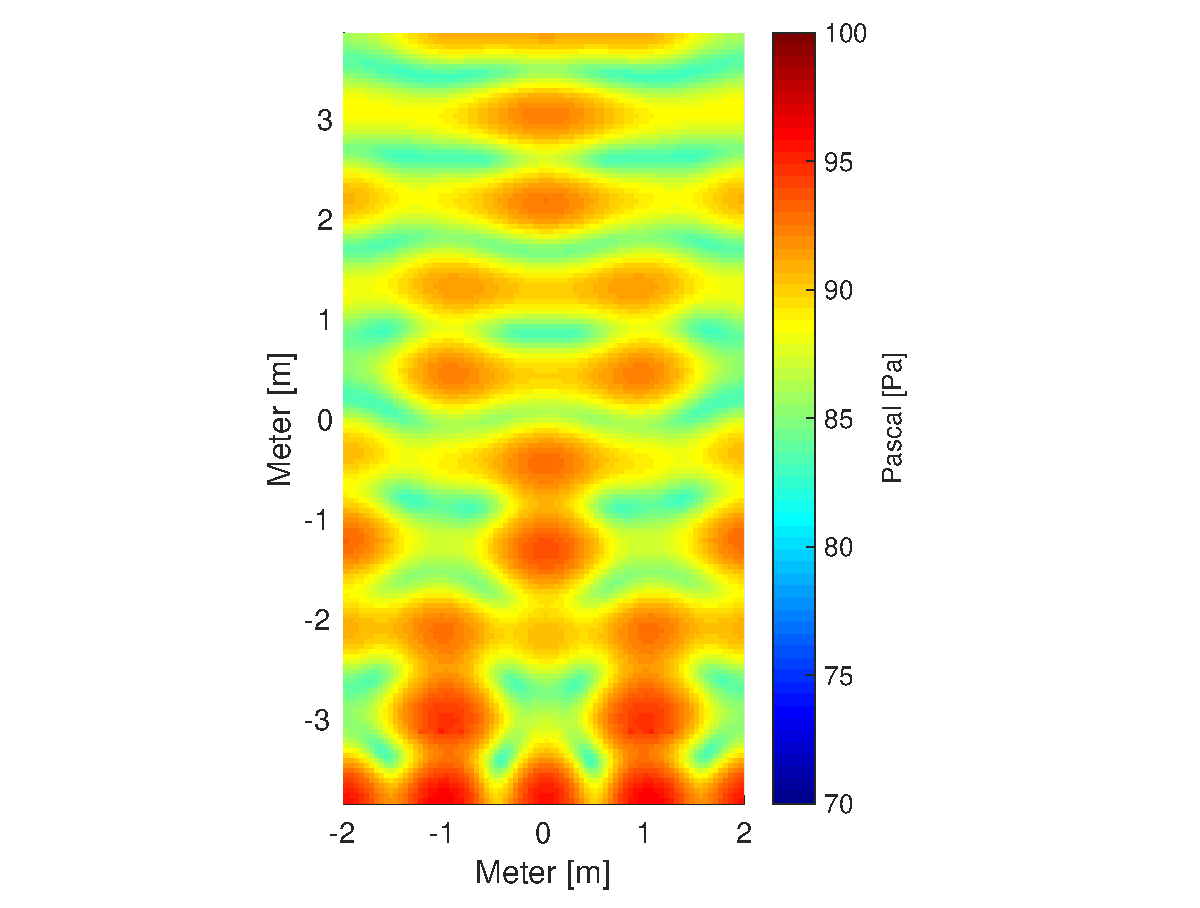
\includegraphics[width=0.95\textwidth]{200_hz_inside_without_beam.eps}
\subcaption{Indoor simulation of  \SI{200}{\hertz} without beamforming}
\label{fig:Indoor_simulation_200_off}
\end{subfigure}
\begin{subfigure}[c]{0.5\textwidth}
\includegraphics[width=0.95\textwidth]{300_hz_inside_beam.eps}
\subcaption{Indoor simulation of  \SI{300}{\hertz} with beamforming}
\label{fig:Indoor_simulation_300_on}
\end{subfigure}
\begin{subfigure}[c]{0.5\textwidth}
\includegraphics[width=0.95\textwidth]{300_hz_inside_without_beam.eps}
\subcaption{Indoor simulation of  \SI{300}{\hertz} without beamforming}
\label{fig:Indoor_simulation_300_off}
\end{subfigure}
\caption{The figure shows a 2 dimension \gls{fdtd} simulation in a room of size  (\SI{4.15}{\meter} x \SI{7.8}{\meter}) where the absorbing coefficient is set to 0.5}
		\label{fig:Indoor_simulation_200_300}
\end{figure}

In \autoref{fig:Indoor_simulation_60_100} and \autoref{fig:Indoor_simulation_200_300} it can be seen that the pressure in the room is not even ether with beamforming active or not. But one notable thing is that the pressure in the room at low frequency with omnidirectional array gets very high compare to higher frequency. So the room amplify the low frequency with reflection more that in the higher frequency area. The pressure seems to be more frequency pressure constant with beamforming active compare to beamforming disabled.\\


A second indoor application is the monitoring. In a monitoring application the room tens to be larger than a living room. The use of monitoring is often at both small and big concert where both dedicated concert hall and sports arenas are used. The following simulating example are done in a sports arena where the spectator area at sports event are on the long side of the playing field. A handball playing field do have a size of (\SI{20}{\meter}x\SI{40}{\meter}) and in this case the spectator is \SI{5}{\meter} on both long side. The following simulation \autoref{fig:Indoor_monitor_60_300} shows a simulation where the stage is placed on the top of the simulation with two monitor. Both monitors is playing upwards when looking at the simulation.


\begin{figure}[H]
\begin{subfigure}[c]{0.5\textwidth}
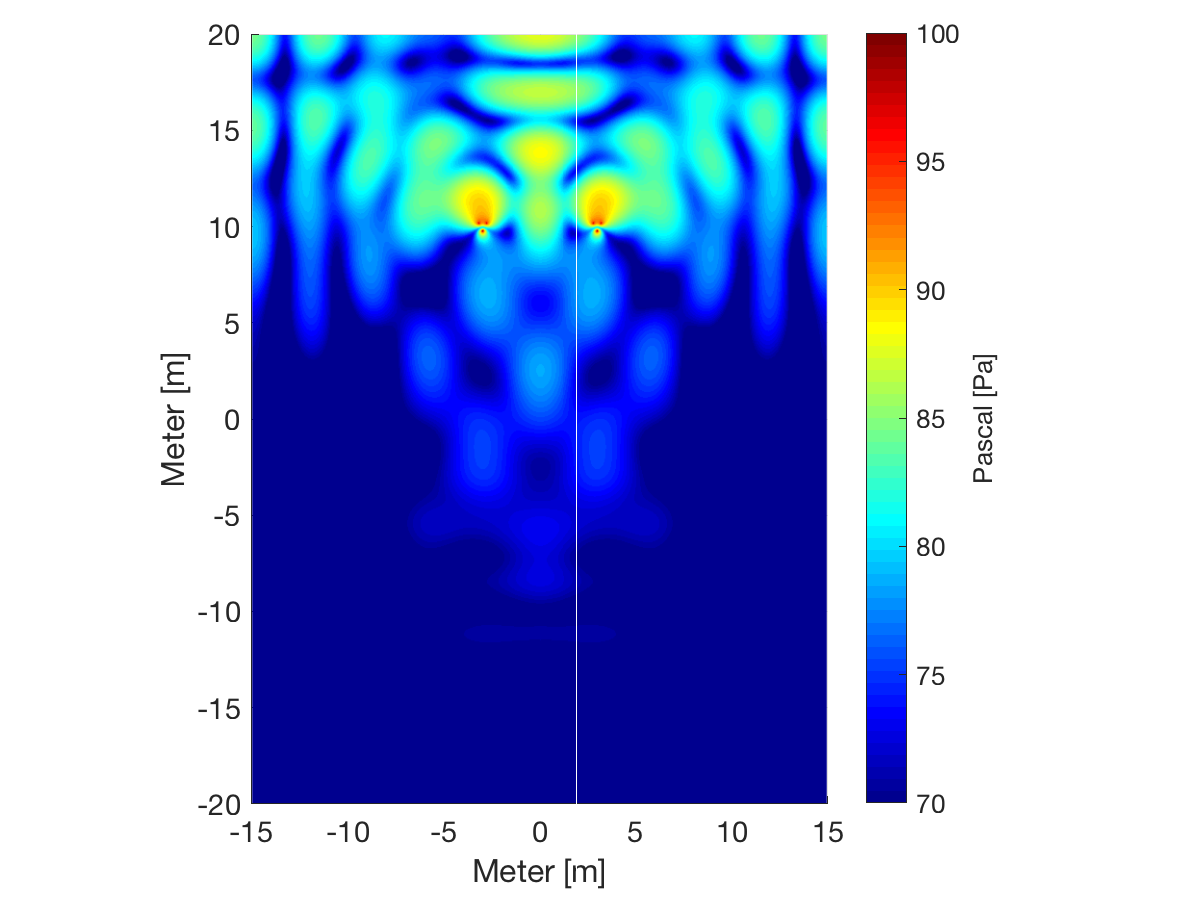
\includegraphics[width=0.95\textwidth]{60_hz_monitor_beam.eps}
\subcaption{Indoor simulation of  \SI{60}{\hertz} with beamforming}
\label{fig:Indoor_monitor_60_on}
\end{subfigure}
\begin{subfigure}[c]{0.5\textwidth}
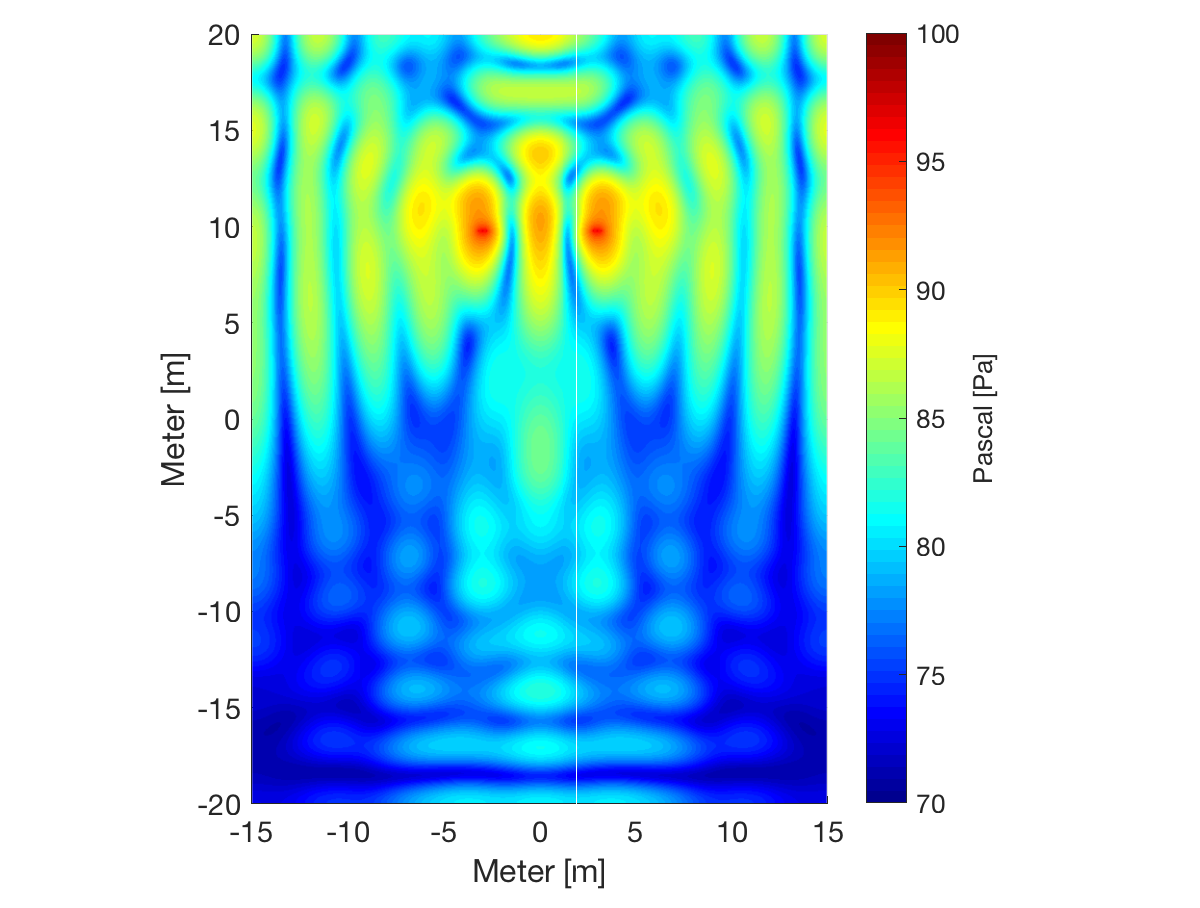
\includegraphics[width=0.95\textwidth]{60_hz_monitor_without_beam.eps}
\subcaption{Indoor simulation of  \SI{60}{\hertz} without beamforming}
\label{fig:Indoor_monitor_60_off}
\end{subfigure}\\
\hspace{0.1\textheight}
\begin{subfigure}[c]{0.5\textwidth}
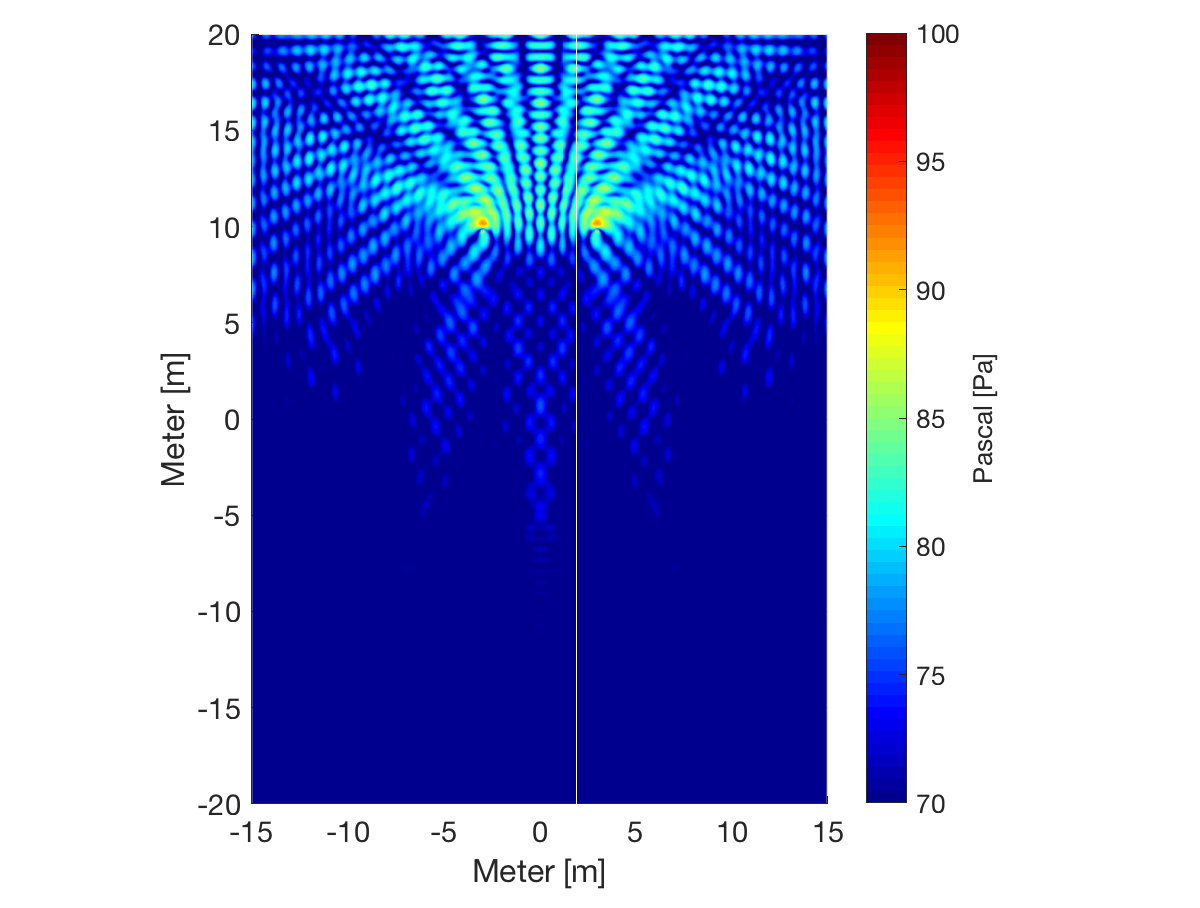
\includegraphics[width=0.95\textwidth]{300_hz_monitor_beam.eps}
\subcaption{Indoor simulation of  \SI{300}{\hertz} with beamforming}
\label{fig:Indoor_monitor_300_on}
\end{subfigure}
\begin{subfigure}[c]{0.5\textwidth}
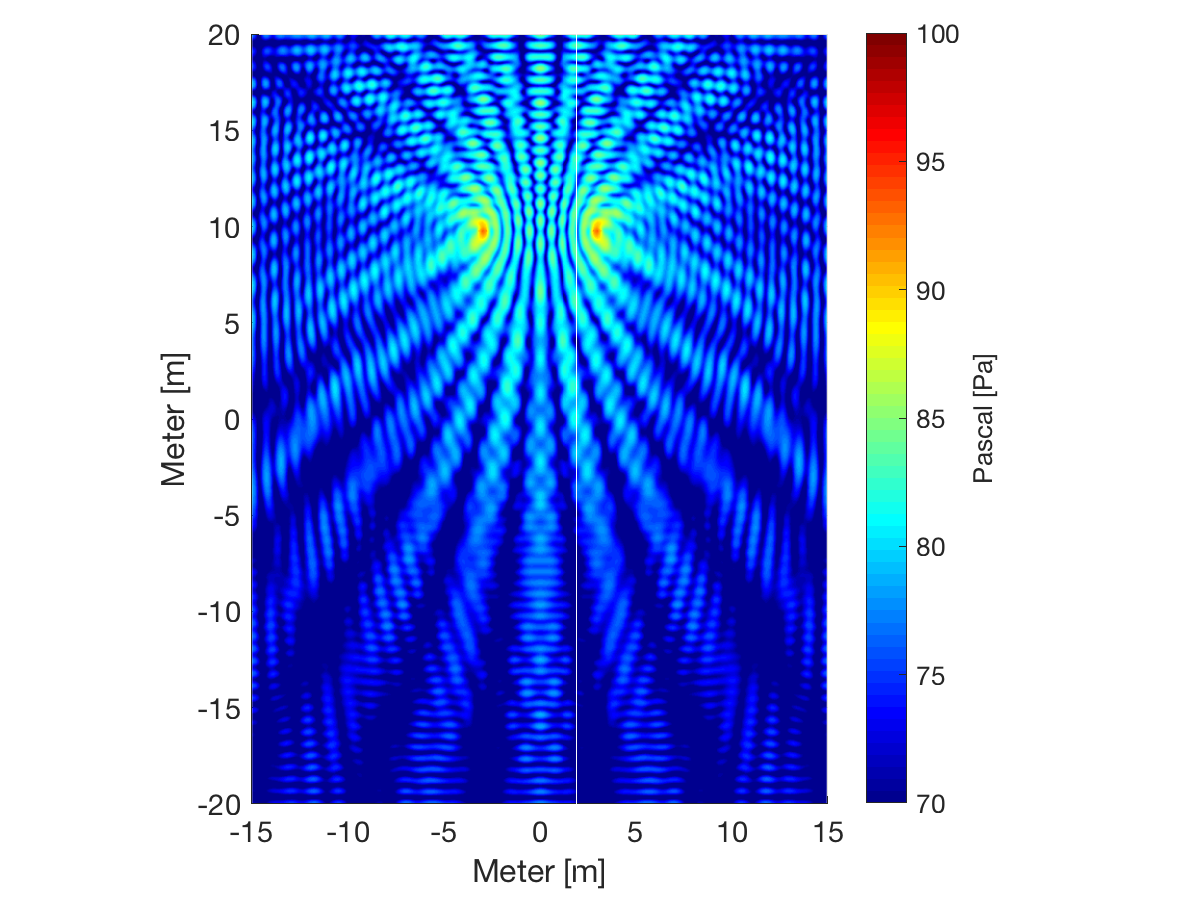
\includegraphics[width=0.95\textwidth]{300_hz_monitor_without_beam.eps}
\subcaption{Indoor simulation of  \SI{300}{\hertz} without beamforming}
\label{fig:Indoor_monitor_300_off}
\end{subfigure}
\caption{The figure shows a 2 dimension \gls{fdtd} simulation in a monitor application where the absorbing coefficient is set to 0.5}
		\label{fig:Indoor_monitor_60_300}
\end{figure}

In \autoref{fig:Indoor_monitor_60_300} it can be seen that the two monitor playing cardioid mostly have an effect on the audience and do not change much on stage. On change to the monitoring system might be that those two monitors was changed with only one beamforming monitor, but feeded with to signals and different beamforming. So one signal is playing to the left of the monitor, there the other signal was playing to the right. This concept have not been tested but it might be one possibility for change of the beamforming system.

 
%

\glsresetall
\appendix % Start of appendix
\addtocontents{toc}{\protect\setcounter{tocdepth}{0}} 
%\input{chapters/appendices/_appendices} % Include appendices
%Appendix:

 \graphicspath{{figures/appendix/}}
\part{Appendix}\label{pt:appendix}
\section{Outline ...}
In this appendix the control of the Outline turntable will be descriped    
